\documentclass{beamer}

\usepackage{presentation}

% The title of the presentation:
%  - first a short version which is visible at the bottom of each slide;
%  - second the full title shown on the title slide;
\title[Compilers]{Topics in Compilers for GATE}

% Optional: a subtitle to be dispalyed on the title slide
\subtitle{Demo Presentation at Vidyalankar}

% The author(s) of the presentation:
%  - again first a short version to be displayed at the bottom;
%  - next the full list of authors, which may include contact information;
\author[Anshuman Dhuliya]{
    Anshuman Dhuliya \\
  {\small \url{anshumandhuliya@gmail.com}} }

% The institute:
%  - to start the name of the university as displayed on the top of each slide
%    this can be adjusted such that you can also create a Dutch version
%  - next the institute information as displayed on the title slide
\institute[Vidyalankar]{
    PhD Scholar At \\
  Indian Institute of Technology Bombay}

% Add a date and possibly the name of the event to the slides
%  - again first a short version to be shown at the bottom of each slide
%  - second the full date and event name for the title slide
\date[Demo PPT Mar 2017]{
  Mar 2017}


\begin{document}
\begin{frame}
    \titlepage
\end{frame}


\begin{frame}
    \frametitle{Outline}
    \tableofcontents[onlyparts]
\end{frame}


\begin{frame}
    \frametitle{About the Presentation}
    \begin{itemize}
        \item The content of the presenation are inspired from [\prettyref{bib:aho1986compilers}].
        \item Many other resources have been used.
        \item Personal material has been added appropriately.
    \end{itemize}

    \onslide<2->{
    \begin{block}{Student Friendly}
        The idea is to create summary slides which the students can quickly refer for revision. These slides can easily be converted to printable handouts.
     \end{block}
}
\end{frame}

\part{Introduction to Compilers}
\frame[plain]{
    \partpage
}
\begin{frame}
  \frametitle{What is a Compiler?}

    \onslide<1->{
  \begin{block}{Basically}
    A compiler is a language translator. It translates from one programming language to another. (E.g. C to Assembly, Java to C, C++ to C)
  \end{block}
  }

    \onslide<2->{
  \begin{block}{We can say...}
    A compiler processes \textit{programming language}. Or in other words, a compiler is a kind of \textit{language} processor.
  \end{block}
  }

\end{frame}

\begin{frame}
  \frametitle{Human translators behave like a Compiler}

\begin{pspicture}(0,0)(124,140) % without grid
    %\psframe(0,0)(62,70)

    \putnode{n1}{origin}{20}{30}{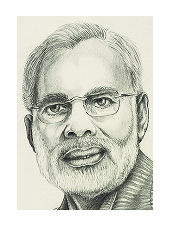
\includegraphics[natwidth=66,natheight=93,width=66pt]{images/modi.eps}}

    \putnode{n2}{origin}{200}{30}{
\includegraphics[natwidth=236,natheight=308,width=66pt]{images/trump.eps}}

    \putnode{n22}{n1}{0}{55}{}
    \putnode{n23}{n2}{0}{55}{}


    \only<2->{\putnode{n3}{origin}{110}{100}{
\includegraphics[natwidth=116,natheight=139,width=66pt]{images/woman.eps}}}

    \only<2->{\putnode{n21}{n3}{-25}{0}{}
    \putnode{n24}{n3}{25}{0}{}}

    \only<1>{\putnode{n7}{origin}{75}{100}{\cfgcode{PM Modi wants to speak in Hindi.\newline{} But Mr. Trump doesn't know Hindi.}}}

    \only<3->{\putnode{n8}{n1}{0}{48}{\cfgcode{Aapko jeet ki bohot badhai.}}}
    \only<3->{\putnode{n9}{n1}{10}{41}{\cfgcode{Aasha hai ham milkar kaam karenge.}}}

    \only<4->{\putnode{n8}{n2}{0}{45}{\cfgcode{Congratulations on the win.}}}
    \only<4->{\putnode{n9}{n2}{0}{38}{\cfgcode{We wish to work together.}}}

    \putnode{n4}{n1}{0}{-38}{\cfgcode{PM Modi}}
    \putnode{n5}{n2}{0}{-35}{\cfgcode{POTUS}}
    \only<2->{\putnode{n6}{n3}{0}{-35}{\cfgcode{Translator}}}

    \only<3->{\nccurve[angleA=45,angleB=180,ncurv=1]{->}{n22}{n21}}
    \only<4->{\nccurve[angleA=0,angleB=90,ncurv=1]{->}{n24}{n23}}

    \only<5->{\putnode{n30}{n3}{0}{-60}{\psframebox[fillstyle=solid,fillcolor=lightgray,opacity=0.8]{She is working like a compiler!}}}

    \only<6->{\putnode{n31}{n3}{60}{40}{\psframebox[fillstyle=solid,fillcolor=lightgray,opacity=0.8]{Meaning is preserved!!}}}
\end{pspicture}


\end{frame}


\begin{frame}
  \frametitle{Compiler}
    \begin{block}{Precisely...}
        Compiler is a software that translates the input language program into a target language program, with equivalent meaning.
    \end{block}
%    \vspace*{\fill}

\begin{pspicture}(0,0)(124,100) % without grid
    %\psframe(0,0)(62,70)
    \putnode{n1}{origin}{110}{70}{\psframebox{\cfgcode{COMPILER}}}

    \putnode{n2}{n1}{-50}{0}{\cfgcode{Source Progarm}}
    \putnode{n21}{n2}{20}{0}{}

    \putnode{n3}{n1}{50}{0}{\cfgcode{Target Program}}
    \putnode{n31}{n3}{-20}{0}{}

    \ncline{->}{n21}{n1}
    \ncline{->}{n1}{n31}

    \only<2->{
    \putnode{n4}{origin}{110}{20}{\psframebox{\cfgcode{INTERPRETER}}}

    \putnode{n5}{n4}{-60}{5}{\cfgcode{Source Progarm}}
    \putnode{n51}{n5}{22}{0}{}

    \putnode{n7}{n4}{-60}{-5}{\cfgcode{Input}}
    \putnode{n71}{n7}{12}{0}{}

    \putnode{n6}{n4}{50}{0}{\cfgcode{Output}}
    \putnode{n61}{n6}{-15}{0}{}

    \ncline{->}{n71}{n4}
    \ncline{->}{n51}{n4}
    \ncline{->}{n4}{n61}
}

\end{pspicture}


\end{frame}


\begin{frame}
  \frametitle{Phases of a Compiler}
    \begin{block}{Compiler is a BIG Algorithm}
        Its is so big that it comprises of hundereds of sub-algorithms. And like any algorithm, Compilers work in a step-by-step fashion. These steps are called phases.
    \end{block}
    \onslide<2->{
    \begin{enumerate}
        \item Lexical Analyzer (covered here)
        \item Syntax Analyzer (partially covered here)
        \item Semantic Analyzer
        \item Intermediate Code Generator
        \item Machine-Independent Optimizer
        \item Target Code Generator
        \item Machine-Dependent Optimizer
    \end{enumerate}
}
\end{frame}


\begin{frame}[fragile]
  \frametitle{Lexical Analysis}
    \begin{block}{}
        Input : \Term{Raw Program}, Output : \Term{Stream of Tokens}
    \end{block}

    \begin{lstlisting}[language=C, frame=leftline,]
int main() { // C program
    int sum;
    sum = 10 + 15 * 6;
}
\end{lstlisting}

    \begin{itemize}
        \item<2-> Lets only consider statement \Codetb{3} for our purpose.
        \item<3-> This program is adding \Codetb{10} with the product of \Codetb{15} and \Codetb{6}, and storing it in an \Codet{int} variable \Code{sum}.
        \item<4-> The smallest logical units on line \Codetb{3} are : \Code{sum}, \Code{=}, \Codetb{10}, \Code{+}, \Codetb{15}, \Code{*}, \Codetb{6} and \Codeb{;}. These are called \textbf{Lexemes}.
        \item<5-> Lexical Analyzer extracts these lexemes and converts them into \textbf{tokens}.
    \end{itemize}
\end{frame}


\begin{frame}
  \frametitle{What are Tokens?}
    \begin{block}{}
        Tokens are generalization of Lexemes.
    \end{block}

    \begin{itemize}
        \item<1-> Tokens provide important information about the lexemes.
        \item<2-> For example, lexeme \Codetb{10} is converted to a token like \texttt{<num, 10>}. Similarly other constants are converted to, \texttt{<num, 15>}, \texttt{<num, 6>}.
        \item<3-> One of the task of Lexical Analyzer is to classify the lexemes. Here, \Codetb{10}, \Codetb{15}, \Code{6} are classified as a number.
        \item<4-> Similarly, \Code{sum} is classified as an \texttt{identifier}. And can be represented as \texttt{<id, sum>}

    \end{itemize}
\end{frame}


\begin{frame}[fragile]
  \frametitle{Input/Output of Lexical Analyzer}
    If input is this line,

    \begin{lstlisting}[language=C, frame=leftline,]
    sum = 10 + 15 * 6;
\end{lstlisting}

    \begin{block}{then lexemes are}
        \DCode{sum} \DCode{=} \DCodetb{10} \DCode{+} \DCodetb{15} \DCode{*} \DCodetb{6} \DCodeb{;}
    \end{block}

    \begin{block}{and tokens are}
        \texttt{<id, sum>}, \texttt{<=, =>}, \texttt{<num, 10>}, \texttt{<+, +>}, \texttt{<num, 15>}, \texttt{<*, *>}, \texttt{<num, 6>}, \texttt{<;, ;>}
    \end{block}

    Lexical Analyzer takes raw program as input and produces a \textit{stream} of tokens. Which is fed to the Syntax Analyzer.

\end{frame}



\begin{frame}
  \frametitle{Syntax Analyzer}
    \begin{block}{}
        Input: \Term{Stream of Token}, Output: \Term{Syntax Tree}

    \end{block}

    \begin{itemize}
        \item<2-> Is the sequence of tokens correct?
        \item<3-> \Codetb{sum = 10 + 15 * 6} is valid, \Codetb{10 + 15 * 6 = sum} is not.
        \item<4-> As English as grammar rules, computer languages have grammar rules too.
        \item<5-> Programs written in any particular language, must follow its grammar rules, otherwise it is an ERROR.

    \end{itemize}
\end{frame}


 % introduction.tex


\part{Predictive Parsing Grammars}
\frame[plain]{
    \partpage
}
\begin{frame}
\frametitle{Properties of Predictive Parsing Grammars}

\begin{enumerate}
\item They are not ambiguous.
\item They are not left recursive (direct or indirect).
\item The FIRST set of each body of a terminal should be disjoint.
\end{enumerate}

\end{frame}


\begin{frame}
\frametitle{Ambiguity}

\begin{block}{Discovering and Removing Ambiguity}
When more than one parse tree can derive the same string of the language, then the grammar is ambiguous.

Proving a grammar ambiguous is an undecidable problem. And there is no algorithm to remove ambiguity from a grammar.

\end{block}

\begin{example}{Ambiguous Grammar}

\texttt{S -> S + S | S - S | 0 | 1 | 2 | 3 | ... | 9}

\vspace{1em}

\texttt{Stmt -> if Expr then Stmt}

\texttt{Stmt -> if Expr then Stmt else Stmt}

\texttt{Stmt -> other}

\end{example}

\end{frame}


\begin{frame}
\frametitle{Eliminating Left Recursion}

\begin{example}{Left Recursion Grammars}
\texttt{E -> E + T}

\texttt{E -> T}

\vspace{1em}

\texttt{A -> Cd}

\texttt{B -> Ce}

\texttt{C -> A | B | f}


\texttt{Stmt -> other}
\end{example}

\begin{block}{Left Recursion can be removed}
Every left-recursive grammar can be converted to a right-recursive grammar.

\vspace{1em}

\texttt{A -> A$\alpha$ | $\beta$}

\vspace{1em}

\texttt{A -> $\beta$A'}

\texttt{A' -> $\alpha$A' | $\epsilon$}

\end{block}

\end{frame}
 % predictiveparsing.tex


\part{Gate Questions}
\frame[plain]{
    \partpage
}
\scriptsize
\begin{frame}
\frametitle{Question 1 : Gate 2017}

\begin{example}
Consider the following expression grammar G:

\texttt{E -> E - T | T}\newline
\texttt{T -> T + F | F}\newline
\texttt{F -> (E) | id}

    Which of the following grammars is \textbf<2->{not left recursive}, but is \textbf<2->{equivalent to G}?

\begin{tabular}{c c}
    \specialcell[t]{(A)\\\texttt{E -> E - T | T}\\\texttt{T -> T + F | F}\\\texttt{F -> (E) | id}}
     & \specialcell[t]{(B)\\\texttt{E -> TE'}\\\texttt{E' -> -TE' |}$\epsilon{}$\\\texttt{T -> T + F | F}\\\texttt{F -> (E) | id}} \\
    \specialcell[t]{(C)\\\texttt{E -> TX}\\\texttt{X -> -TX |} $\epsilon$\\\texttt{T -> FY}\\\texttt{Y -> +FY | }$\epsilon$\\\texttt{F -> (E) | id} }
    & 
    \specialcell[t]{(D)\\\texttt{E -> TX | (TX)}\\\texttt{X -> -TX | +TX |} $\epsilon$\\\texttt{T -> id}}
\end{tabular}

\end{example}
\end{frame}

\begin{frame}
\frametitle{Question 2 : Gate 2005}

\begin{example}
    The grammar \texttt{A -> AA | (A) | } $\epsilon$ is \textbf<2->{not suitable for predictive-parsing} because the grammar is:


   \vspace{3em}

    (A) Ambiguous

    (B) Left-recursive

    (C) Right-recursive

    (D) An operator-grammar

\end{example}
\end{frame}


\begin{frame}
\frametitle{Question 3 : Gate 2009}

\begin{example}
    Which data structure in a compiler is used for managing information about variables and their attributes?

   \vspace{3em}


    (A) Abstract syntax tree

    (B) Symbol table

    (C) Semantic Stack

    (D) Parse table

\end{example}
\end{frame}


\begin{frame}
\frametitle{Question 4 : Gate 2010}

\begin{example}
    The grammar \texttt{S -> aSa | bSc | c} is,

   \vspace{3em}


    (A) LL(1) but not LR(1)

    (B) LR(1) but not LL(1)

    (C) Both LL(1) and LR(2)

    (D) Neither LL(1) nor LR(1)

\end{example}
\end{frame}


\begin{frame}
\frametitle{Question 5 : Gate 2014}

\begin{example}
    Consider the grammar defined by the following productoin rules, with two operators \texttt{*} and \texttt{+}

    \texttt{S -> T * P}

    \texttt{T -> U | T * U}

    \texttt{P -> Q + P | Q}

    \texttt{Q -> id}

    \texttt{U -> id}

   \vspace{3em}

    (A) + is left associative, while * is right associative

    (B) + is right associative, while * is left associative

    (C) Both + and * are right associative

    (D) Both + and * are left associative


\end{example}


\end{frame}

\normalsize
 % gatequestions.tex


\begin{frame}[plain]
    \begin{center}
        \textbf{\Huge{}Thank You}
    \end{center}
\end{frame}


\begin{frame}[t,allowframebreaks]
        \frametitle{References}
        \printbibliography
        % \bibliographystyle{ieee}
        % \bibliography{references}
\end{frame}


\end{document}


